%!TEX root = ThesisLKN.tex
\chapter{Introduction}

In recent years, more and more robots are deployed in not only industrial environments but also human populated areas. In order to fulfill their tasks, it is necessary for robots to interact and even cooperate with people. Therefore, tracking the locations of people in those environments has gained enormous attentions in robotics community. Besides, with the increasing popularity of artificial intelligence, robots are also expected to be intelligent enough to predict possible future locations of walking human even when encountered with occlusions or missing of sensor data. Enabled with an accurate tracking and prediction of human movements, robots are able to have a better understanding of the environment, which will facilitate interactions between robots and human.

The very fist requirement for a robot to operate is to model the environment. A simple yet effective way is to use occupancy grid map representation of the environment \citep{moravec1985high}. It decomposes the environment into cells with a predefined resolution, and the state of each cell is either \textit{occupied} or \textit{not occupied}. This representation has been extensively used in many different kind of robot tasks like simultaneous localization and mapping (SLAM). The classical grid map representation treats the environment as static, which is not always the case in real scenarios. In other words, the environment can be dynamic since objects can move around in the environment. Object tracking addresses dynamics in environment explicitly, since it tracks and predicts how objects move. If there are more than one object involved at the same time, the tracking problem becomes multiple object tracking (MOT). In people tracking systems, the dynamics in environment refer to people location changes along the time horizon (i.e., trajectories). 

Commonly, a tracking system is implemented as a multiple stage pipeline, which consists of object detection, data association, motion modeling and occupancy generation. When deal with a multiple object tracking problem, data association becomes very tricky. The classical way to perform data association is to maintain a list of known objects, and associates new observations with those objects. The main difficulty of this approach is to deal with \textit{birth} (whether observation is from a new object) and \textit{death} (whether a maintained object should be deleted) of tracks explicitly \citep{gauvrit1997formulation}. 

To address the data association problem, \citet{coue2006bayesian} proposed \textit{Bayesian occupancy filter} (BOF), which is an object tracking algorithm based on grid map representation of environment. It essentially avoids data association step in the tracking pipeline, since concepts of \textit{objects} and \textit{tracks} dose not exist in BOF framework. Rather than treat tracking problem from an \textit{object} point of view, BOF addresses tracking from a \textit{cell} perspective. That is to say, tracks are replaced by transitions of occupancies between cells over time. Meanwhile, BOF is robust to object occlusion thanks to the combination of \textit{prediction} and \textit{estimation} steps. This two-step mechanism is well suited for handling the consistency between occupancy predictions and past observations, therefore uncertainties incurred by occlusion is naturally handled in a probabilistic way. Over the past few years, there has been some extensions over BOF proposed in literature \citep{gindele2009bayesian, brechtel2010recursive, llamazares2013dynamic}. 

\begin{figure}[H]
  \centering
    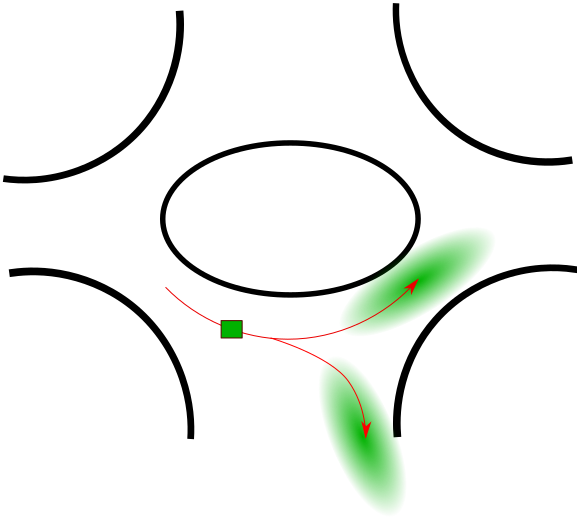
\includegraphics[width=.5\textwidth]{figures/roundabout.png}
    \caption[An illustration of a round-about]{This shows an illustration of a round-about. Cars can only drive in directions indicated by red arrows. The green rectangle represents a car at that location. Since we know that the car must drive in the specified directions, the possible locations of the car after a few time steps are indicated by the two green eclipses. This prior knowledge helps us track the dynamic objects since we have better chances to locate the car according to the motion pattern.}
    \label{fig:roundabout_idea}
\end{figure}

A tracking system usually predicts the state of the world (e.g., object location and velocity) based on past observations. Many tracking algorithms also incorporate motion models of the objects being tracked, since this allows us to utilize prior knowledge of object's motion cues. As an intuitive example, let us consider a round-about as shown in Figure \ref{fig:roundabout_idea}, where cars can only drive in one direction. To track a car driving in a round-about, prediction of next possible locations of the car should always be on the side which allowed driving direction indicates, since we know that the car must follow that direction. Likewise, human tracking in indoor environments can also benefit from human motion patterns. For BOF and its variants, the objects being tracked are assumed to perform linear motion, which indicates that objects always move in the same direction as in the last time step. Although \citet{gindele2009bayesian} proposed to incorporate prior map knowledge (BOFUM) to better model the motion dynamics based on cell context, linear motion is too simplistic to model actual human motion in indoor environments. 

Based on our observations of human trajectories, we found two aspects very important for explaining human motion: 1) Unlike in free space, people have to move under spatial constraints in indoor environments. For example, people tend to walk along the central area between walls in a corridor and change their walking directions when they have to make turns. That is to say, the spatial constraints limit human motion patterns and therefore human motion is very place dependent. 2) People move continuously in time and space, which means they does not disappear or appear out of thin air. If a person is currently at a cell of a grid map, he or she has to walk through its neighboring cells first. In other words, future movement events starting from a region of interests are highly influenced by state changes of its neighboring cells. These observations motivates us to model human motion in a way that captures both \textbf{place dependency} as well as \textbf{spatial correlation} between cells.

In computer vision community, researches in machine learning over last few years has shown a lot of successes. Image classification algorithms based on convolutional neural networks (CNNs) has won all ImageNet classification challenges since 2012 \citep{russakovsky2015imagenet}. Researches show that the depth of network plays a very important role in CNNs' performance. However, deep networks are more difficult to train due to poor gradient flow during back-propagation. Thanks to the development of ResNet \citep{he2016deep} and DenseNet \citep{huang2016densely}, the state-of-the-art CNNs can be as deep as over 1000 layers without training difficulties. Besides, fully convolutional neural networks \citep{long2015fully} are proven to be very powerful in solving semantic segmentation tasks thanks to its pixel-to-pixel classification ability. \citet{jegou2017one} extends the DenseNet to a fully convolutional neural network with an upsampling path for dealing with the problem of semantic segmentation. 

It turns out that CNNs can achieve good results in not only computer vision tasks but also many other domains. For example, recurrent neural networks (RNNs) can be applied in automatic language translation \citep{cho2014learning}. Deep reinforcement learning are good choice for teaching robots to perform human actions like grasping\citep{levine2016learning}. Essentially, the reason why CNN works in those domains is that it is able to capture complex structure in data. Once a CNN learns that structure, it can generalize to cases that never occurs during training. Therefore, if we feed a gird map as input and human motion patterns as ground truth to a network, it should be able to learn the patterns after training with lots of data. We model human motion patterns as a set of conditional probabilities for every cell on the map. They represent how likely a person moves to one of the neighboring cells, conditioned on which neighboring cell he or she comes from. Since these probabilities incorporate information about the incoming cell, the motion model captures spatial correlations between cells. Besides, they are different for each cell based on cell's context on the map, which means the learned motion pattern is expressive enough to predict different motions at different locations. In other words, our motion model is place dependent. In fact, similar idea of modeling motion patterns has been proposed by \cite{kucner2013conditional}, but they need sensor observations from the map to learn motion pattern on that map. On the contrary, we exploit the power of CNNs so that our method can generalize to maps that have never occurs.

\begin{figure}[H]
  \centering
    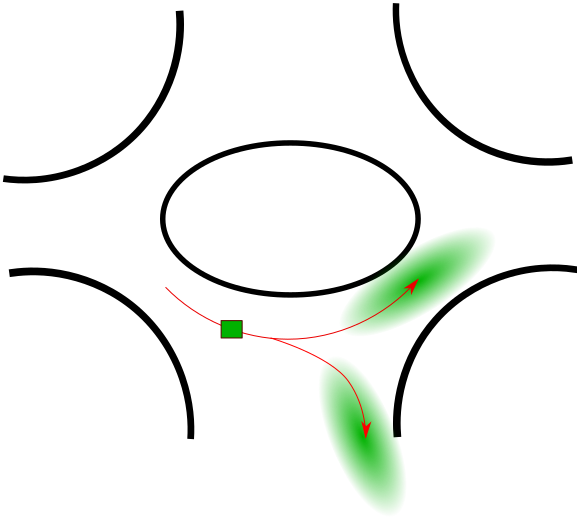
\includegraphics[width=.5\textwidth]{figures/roundabout.png}
    \caption[An example of future occupancy predictions of our method.]{An example of future occupancy predictions of our method.  The map shows a T-section, where only white spaces are walkable. Initially, a person is shown as a red rectangle and with velocity towards left. Since no further sensor reading is given, BOFMP propagates occupancies over time. After some time interval, most occupancies appear in both upper and lower branches of the corridor, which proves that our motion model successfully learns that people tend to make turns at the intersection. Besides, our BOFMP predicts more occupancies in the middle of corridors, since it learns that people are less likely to walk near walls.}
    \label{fig:idea}
\end{figure}

The data we use for training network is generated from simulated human walking trajectories on SLAM-generated maps of real world offices. Once the network finishes learning, we can feed new maps to the network and obtain human motion patterns from network outputs. These motion patterns are then incorporated into BOF framework to perform human tracking in indoor environments. We call our tracking method as \textit{Bayesian Occupancy Filter with Motion Patterns} (BOFMP). If only initial state of a person is given and no further observations are provided, our method is able to predict reachable areas after some time steps. Figure \ref{fig:idea} shows an example of future occupancy predictions of our method without sensor observations. It shows that our way of modeling human motion patterns enables BOF to propagate occupancies to reasonable areas.

The main contributions of this thesis work are:

\begin{my_enumerate}
\item We present a way of modeling human motion patterns that captures both place dependency and spatial correlations between cells. Besides, thanks to powerful generalization abilities of CNNs, our method can generate motion patterns on maps that are never seen by our model.
\item We incorporate the learned motion patterns into BOF framework seamlessly for human tracking in indoor environment, and achieve better tracking performance than baseline method.  The whole pipeline of modeling motion pattern and tracking presented in this thesis work can be applied in other scenarios, such as car tracking in ADAS systems.
\end{my_enumerate}


The rest of this thesis is organized as follows: Chapter \ref{chapter:2} summarizes the related works and highlights the similarities and differences between our method and others in literatures. Chapter \ref{chapter:3} introduces how BOF is derived and mathematical formulation of CNNs. Chapter \ref{chapter:4} explains the detailed implementations, such as generation of dataset and BOF. Chapter \ref{chapter:5} summarizes the dataset and presents the tracking performance of our method and the baseline. Chapter \ref{chapter:6} concludes the thesis work and presents possible improvements on our method. 
